\documentclass{article}
\usepackage{tikz} 
\usepackage{pgfplots} 
\usepackage{stix}
\usepackage{gillius}
\usepackage{ccicons}

\usepackage[margin=0in, includehead, includefoot, paperwidth=8.625in, paperheight=8.75in]{geometry}
\usetikzlibrary{backgrounds}
\usetikzlibrary{patterns}
\renewcommand{\d}{\mathop{}\!d}


\definecolor{scarlet}{RGB}{187,0,0}

\begin{document}
\pagenumbering{gobble}


\tikz[remember picture,overlay] \node[inner sep=0pt] at (current page.center){\includegraphics[height=8.75in]{starsAmber.jpg}};
%\tikz[remember picture,overlay] \node[inner sep=0pt] at (current page.center){\includegraphics[width=8.625in]{frontTemplate.png}};

\flushright

\begin{tikzpicture}[opacity=1]
  \node at (-.8,0) {\scalebox{4}{\Huge\textsf{\textbf{\textcolor{white}{calculus}}}}};
  \node at (8,.2) {\scalebox{10}{\Huge\textsf{\textbf{\textcolor{white!65!black}{\textit{e}}}}}};  %% Aligned with subtitle
  %\node at (8,1.85) {\scalebox{10}{\Huge\textsf{\textbf{\textcolor{white!65!black}{1}}}}}; %% Aligned with title
  \node at (-.7,-1.6) {\resizebox{4.8in}{.2in}{\Huge\textsf{\textcolor{white!65!black}
          {with free online interactive materials}
    }}};
    %\draw[yellow] (-9,-1.2)--(9,-1.2); %guide line
\end{tikzpicture}\hspace*{.3in}

\vspace{1in}

 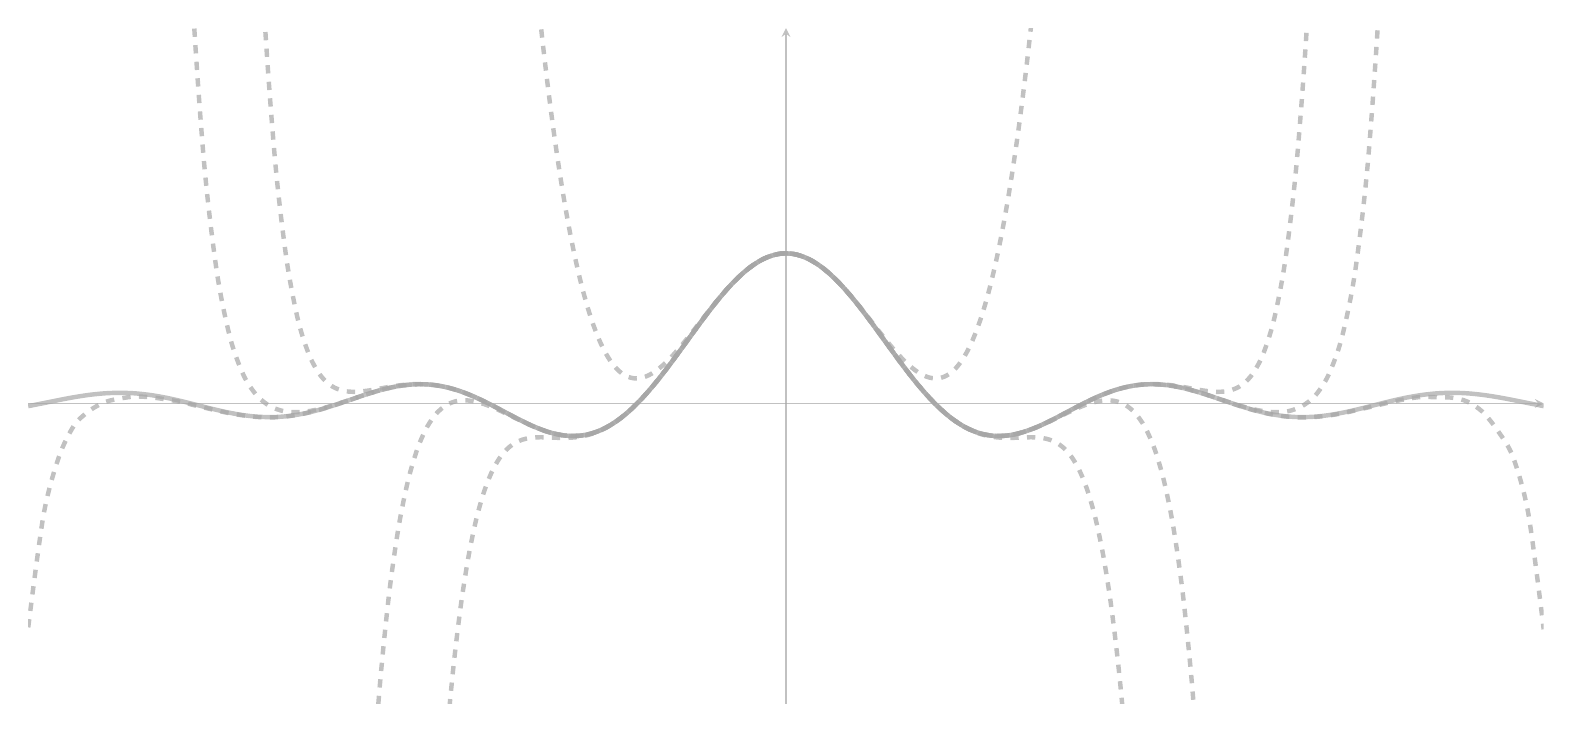
\begin{tikzpicture}[opacity =.7,declare function = {f(\x) = sin(deg(\x))/\x;}]]
    \begin{axis}[
        xmin=-16,
        xmax=16,
        ymin=-2,
        ymax=2.5,
        width=8.2in,
        height=4in,
        axis lines=middle, %xlabel=$x$, ylabel=$y$,
        every axis y label/.style={white!65!black,at=(current axis.above origin),anchor=south},
        every axis x label/.style={white!65!black,at=(current axis.right of origin),anchor=west},
        ticks=none,
        axis line style={white!65!black},
      ]
     
      %% Taylor
      \addplot [ultra thick,dashed, white!65!black, smooth,samples=100,domain=-6:6] {1. -0.166667 *x^2+0.00833333 *x^4}; %% 
      \addplot [ultra thick,dashed, white!65!black, smooth,samples=100,domain=-8:8] {1. -0.166667 *x^2+0.00833333 *x^4-0.000198413 *x^6+2.75573*10^(-6) *x^8-2.50521*10^(-8) *x^10};
      \addplot [ultra thick,dashed, white!65!black, smooth,samples=100,domain=-10:10] {1. - 0.166667*x^2 + 0.00833333*x^4 - 0.000198413*x^6 + 2.75573*10^(-6)*x^8 - 2.50521*10^(-8)*x^10 + 1.6059*10^(-10)*x^12 - 7.64716*10^(-13) *x^14};
      \addplot [ultra thick,dashed, white!65!black, smooth,samples=100,domain=-12:12] {1. -0.166667*x^2+0.00833333*x^4-0.000198413*x^6+2.75573*10^(-6)*x^8-2.50521*10^(-8) *x^10+1.6059*10^(-10)*x^12-7.64716*10^(-13) *x^14+2.81146*10^(-15) *x^16-8.22064*10^(-18) *x^18+1.95729*10^(-20)*x^20};
      \addplot [ultra thick,dashed, white!65!black, smooth,samples=100,domain=-14:14] {1. -0.166667 *x^2+0.00833333 *x^4-0.000198413* x^6+2.75573*10^(-6)* x^8-2.50521*10^(-8)* x^10+1.6059*10^(-10)* x^12-7.64716*10^(-13)* x^14+2.81146*10^(-15)* x^16-8.22064*10^(-18)* x^18+1.95729*10^(-20)* x^20-3.86817*10^(-23)* x^22+6.44695*10^(-26)*x^24};
      \addplot [ultra thick,dashed, white!65!black, smooth,samples=100,domain=-16:16] {1. -0.166667* x^2+0.00833333* x^4-0.000198413* x^6+2.75573*10^(-6)* x^8-2.50521*10^(-8)* x^10+1.6059*10^(-10)* x^12-7.64716*10^(-13)* x^14+2.81146*10^(-15)* x^16-8.22064*10^(-18)* x^18+1.95729*10^(-20)* x^20-3.86817*10^(-23)* x^22+6.44695*10^(-26)* x^24-9.18369*10^(-29)* x^26+1.131*10^(-31)* x^28-1.21613*10^(-34)* x^30+1.15163*10^(-37)* x^32-9.67759*10^(-41)* x^34};
      
      \addplot [ultra thick, white!65!black, smooth,samples=100,domain=-16:16] {f(x)}; %% sinc
     \end{axis}
  \end{tikzpicture}\hspace*{.6in}

\vfill

\flushleft
\hspace*{.4in}\begin{tikzpicture}
  \node at (0,0) {\scalebox{1}{\Huge\textsf{\textcolor{white}{\ccbyncsa}}}};
  \node at (4,-.2) {\large\textsf{\textcolor{white}{developed in \textbf{XIMERA}}}};
\end{tikzpicture}
\vspace*{.2cm}

\end{document}


